\documentclass[../../main.tex]{subfiles}

% 

\begin{document}
\chapter{Polohovo citlivé detektory}

\section{Proporcionálne polohovo citlivé detektory}
Proporcionálny detektor je typ plynového ionizačného detektora používaného na meranie častíc ionizujúceho žiarenia. Kľúčovým prvkom je jeho schopnosť merať energiu dopadajúceho žiarenia tým, že produkuje výstup detektora, ktorý je úmerný energii žiarenia, odtiaľ meno detektora. Pri správnej voľbe napätia sú elektróny, ktoré sa vytvoria v ionizácii, urýchľované smerom k anóde a môžu spôsobiť sekundárnu ionizáciu. V plyne tak môže dôjsť k zosilneniu pôvodného signálu faktorom $\sim 10^4 - 10^6$.

\subsection{Proporcionálna trubica}
Vzhľadom k tomu, že vzniknutá lavína v detektoroch, je obmedzená na malú časť dĺžky anódy, boli vyvinuté schémy, vďaka ktorým je možné tieto detektory použiť k pozične citlivému meraniu udalosti. V bežnej valcovej geometrii detektora, elektróny driftujú z miesta ich vzniku pozdĺž radiálneho poľa k anóde. Poloha lavíny je tak dobrým indikátorom axiálnej pozície, kde bol vytvorený pôvodný iónový pár. Pokiaľ ale dráha ionizujúcej častice smeruje pozdĺž anódy, tak bude okolo anódy rozložených viacej lavín, z čoho je možné určiť len strednú polohu častice. Najbežnejšia metóda snímania polohy v proporcionálnych trubiciach je založená na princípe rozdelenia náboja, viď obrázok (\ref{em9:fig:propor}).

\begin{figure}[!h]
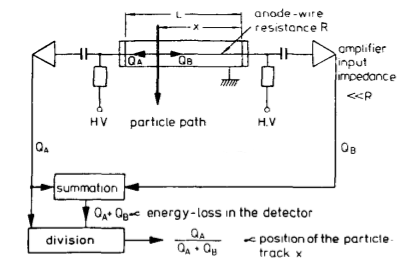
\includegraphics[width=0.9\textwidth]{emsf-09-propor.png}
\centering
\caption{Všeobecná schéma snímania polohy v proporcionálnych trubiciach.}
\label{em9:fig:propor}
\end{figure}

Anódový drôt je vyrobený tak, že má význačný odpor na jednotku dĺžky, takže zozbieraný náboj je rozdelený medzi zosilňovače umiestnené na oboch koncoch drôtu v pomere, ktorý je jednoducho spojený s polohou interakcie. Súčet výstupu obidvoch zosilňovačov vytvára konvenčný výstupný impulz s amplitúdou proporcionálnou k celkovému náboju. Signál polohy sa generuje vydelením výstupu jedného zosilňovača súčtom signálov, aby sa získal impulz, ktorý indikuje relatívnu polohu pozdĺž anódového vodiča.

\subsection{Mnoho-vláknový proporcionálny čítač}
V niektorých situáciách je výhodné dať viac ako jeden anódový drôt do proporcionálneho čítača. Napríklad detektory s veľmi veľkou povrchovou plochou môžu byť konštruované tak, že umiestníme mriežku anódových drôtov medzi dve veľké ploché dosky, ktoré slúžia ako katódy na oboch stranách počítadla. Na obrázku (\ref{em9:fig:multiware}) je načrtnutá táto konfigurácia spoločne s výsledným elektrickým poľom.

\begin{figure}[!h]
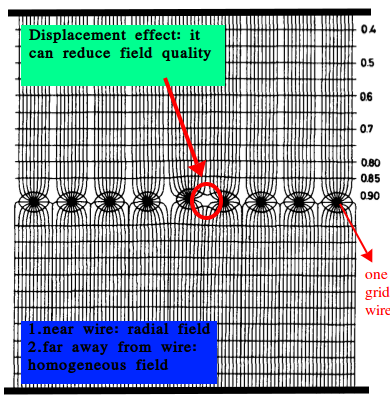
\includegraphics[width=0.6\textwidth]{emsf-09-multiware.png}
\centering
\caption{Graf elektrického poľa vytvorený mriežkou anódových vlákien, ktoré sú umiestnené rovnomerne medzi dvoma paralelnými katódovými doskami v hornej a spodnej časti obrázka. Vo veľkej časti objemu je pole takmer rovnomerne rozložené. V bezprostrednej blízkosti každého sieťového drôtu sa vytvorí oblasť s vysokým poľom.}
\label{em9:fig:multiware}
\end{figure}

Elektróny tvorené ionizáciou plynu driftujú smerom dovnútra k rovine anódových drôtov najprv v takmer rovnomernom poli. Ako sa tak tieto elektróny približujú k anódovej rovine začnú zrýchľovať smerom k najbližšiemu anódovému drôtu. Silné elektrické pole v blízkom okolí anódového drôtu urýchli elektróny natoľko, že dôjde k vytvoreniu elektrónovej lavíny. Na anódovom drôte, na ktorom sa zhromažďuje elektrónová lavína, sa objaví veľký pulz indukovaný negatívnou polaritou, zatiaľ čo susedné anódy vykazujú menšie kladné amplitúdové impulzy. Signály z predzosilňovačov pripojených ku každému drôtu sa teda môžu použiť na lokalizáciu udalosti na najbližší vodič, pričom najmenšia vzdialenosť medzi drôtmi je obmedzená na približne $1-2$ mm.

Katódové roviny môžu byť tiež vyrobené vo forme izolovaných pásikov alebo skupín drôtov, ako je to znázornené napríklad na obrázku (\ref{em9:fig:strip}) alebo (\ref{em9:fig:mnohovlakna}). Pozitívne signály sú vyvolané lavínami na katódových pruhoch, ale keďže sú umiestnené v určitej vzdialenosti, indukovaný náboj je rozložený na širšiu oblasť. Pásy na jednej katódovej rovine môžu byť v smere x, zatiaľ čo pásy na protiľahlej katóde sú často kolmé na prvú rovinu, aby poskytli nezávislú súradnicu y. Zariadenie s takýmto dizajnom môže slúžiť ako polohový detektor, ktorý sa používa pri výskume častíc s vysokou energiou.

\begin{figure}[!h]
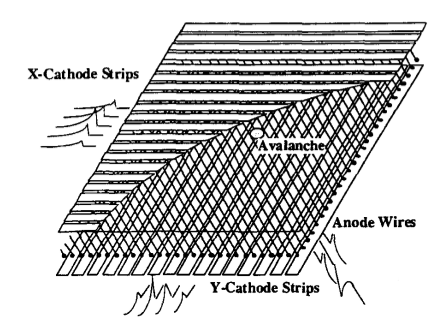
\includegraphics[width=0.6\textwidth]{emsf-09-strip.png}
\centering
\caption{Náčrt dvoj-dimenzionálneho pozične citlivého viac-drôtového proporcionálneho čítača.}
\label{em9:fig:strip}
\end{figure}
\begin{figure}[!h]
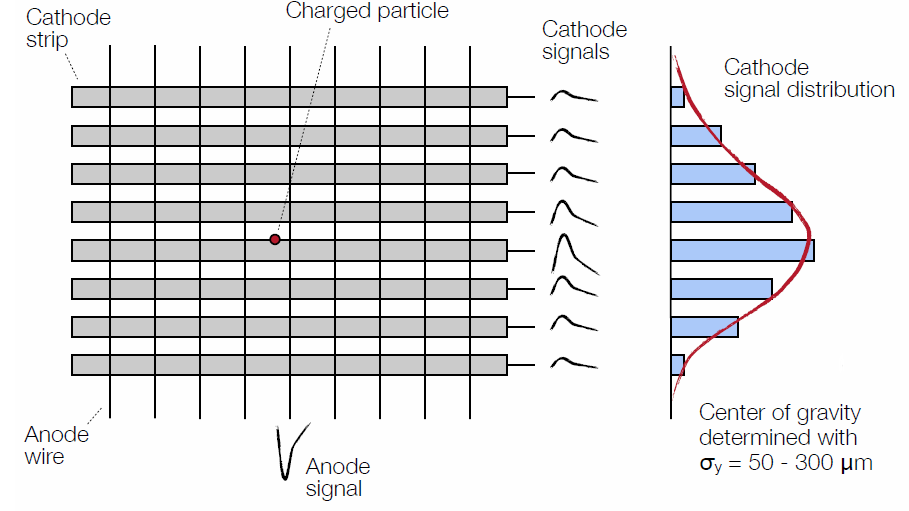
\includegraphics[width=0.9\textwidth]{emsf-09-mnohovlakna.png}
\centering
\caption{Schéma funkcie dvoj-dimenzionálneho proporcionálneho čítača.}
\label{em9:fig:mnohovlakna}
\end{figure}

\subsection{Mikrostripová plynová komora}
Tento typ multi-anódového, plynom plneného detektora bol navrhnutý v roku 1988, aby prekonal nejaké obmedzenia predošlého typu detektora. Hlavnou vlastnosťou tohto typu detektora je to, že rovnako ako u predošle spomenutých typov detektorov sú anódy umiestnené tesne blízko seba (typicky $\sim 10\,\mu m$). Takže rovnaký typ koncentrácie elektrického poľa, ktorý sa vyskytuje okolo drôtu, sa realizuje aj blízko povrchu anódového pásika. Preto, keď sa v tesnej blízkosti tohto anódového pásu ocitnú elektróny, tak sa začnú vytvárať elektrónové lavíny presne takým istým spôsobom, akým sa to dialo v predchádzajúcich detektoroch okolo drôtu.

Príklad kompletnej mikrostripovej plynovej komory je znázornený na obrázku (\ref{em9:fig:mikrostrip}). Oblasť medzi katódovou driftovou rovinou a anódami obsahuje plniaci plyn, v ktorom sa po prechode žiarenia vytvoria iónové páry. Elektróny z týchto iónových párov sa nasmerujú na anódy pomocou elektrického poľa, ktoré  sa vytvorí medzi anódami a katódovou driftovou rovinou. Akonáhle sa tieto driftové elektróny dostanú do bezprostrednej blízkosti povrchu anódy, začnú sa vytvárať lavíny a práve z týchto lavín vzniká takmer všetok detekovaný náboj. 

Nahradenie drôtov kovovými pásmi má zrejmé výhody. Prostredníctvom fotolitografického procesu môžu byť pásy vytvorené s veľmi úzkym rozostupom, takže priestorové rozlíšenie môže byť oveľa jemnejšie ako pri mnoho-drôtových proporcionálnych čítačoch. Ďalšou výhodou je, že väčšina pozitívnych iónov vytvorených v lavíne sa rýchlo priťahuje k blízkym katódam namiesto toho, aby museli driftovať cez celý objem detektora na povrch oveľa vzdialenejšej katódy. Zodpovedajúci pozitívny náboj sa preto rýchlejšie vyčistí z objemu detektora, čo umožňuje oveľa vyššiu rýchlosť prevádzky miktorstripových komôr v porovnaní s drôtovými komorami.

\begin{figure}[!h]
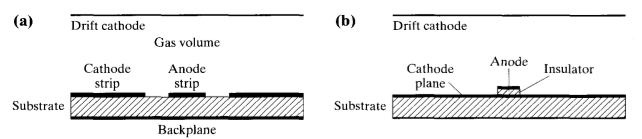
\includegraphics[width=1.0\textwidth]{emsf-09-mikrostrip.png}
\centering
\caption{Prierez mikrostripovej plynovej komory. Časť (a) znázorňuje bežný vzor striedajúcich sa anódových a katódových pásov. Časť (b) ukazuje komoru, kde sú úzke anódové pásy oddelené od spojitej katódovej roviny izolátorom.}
\label{em9:fig:mikrostrip}
\end{figure}

V najbežnejšej konfigurácii zobrazenej na obrázku (\ref{em9:fig:mikrostrip}a) sú striedajúce sa anódové a katódové pásy nanesené na izolačnom substráte. Potenciálnym problémom by mohlo byť, keby substrát tiež zhromažďoval nejaký náboj, čo by mohlo následne viesť k možnému nahromadeniu povrchového náboja, čo by spôsobovalo nestabilitu napätia a deformáciu elektrického poľa. Aby sa zabránilo tomuto nabíjaniu povrchu, musí mať substrát určitú konečnú elektrickú vodivosť. Ďalšou potenciálnou nevýhodou je skutočnosť, že elektrické iskrenie sa môže ľahko vyskytovať medzi anódami a katódami kvôli ich malým rozostupom. Tieto výboje môžu fyzicky poškodiť štruktúru elektród a nakoniec spôsobiť trvalé poškodenie detektora.

Alternatívna štruktúra je tiež uvedená na obrázku (\ref{em9:fig:mikrostrip}b). Tu je katóda spojitým vodičom a anódy sú nesené nad povrchom katódy pričom tieto anódy a katódy sú oddelené izolačnými pásikmi. Táto štruktúra poskytuje lepšie zabezpečenie od iskrenia medzi katódami a anódami.

\section{Polovodičové polohovo citlivé detektory}
Detektory, v ktorých je snímaná poloha interakcie dopadajúceho žiarenia spolu s energiou, majú aplikáciu v mnohých rôznych oblastiach. Dva hlavné typy detektorov, ktoré sa používajú na detekciu polohy nabitých častíc, sú plynové proporcionálne trubice (spomenuté vyššie) a detektory silikónových alebo germániových polovodičových diód. Tieto polovodičové detektory sú niekedy uprednostňované z dôvodu kompaktnosti a nízkej energie, ktorá je potrebná na vytvorenie ión-elektrón páru v porovnaní s detektormi naplnenými plynom. 

\subsection{Pásikový polovodičový polohový detektor} 
V najjednoduchšej forme sa pozične citlivý polovodičový detektor skladá z jedno-dimenzionálno kremíkového či germániového pásika, ktorého jeden kontakt má značný odpor. Ako môžme vidieť na obrázku (\ref{em9:fig:polpasik}), jeden koniec tohto kontaktu je uzemnení a druhý koniec vedie k zosilňovaču pre odvodenie pozičného signálu (P). Kontakt s odporom sa správa ako delič náboja a množstvo náboja doručeného k pozičnému zosilňovaču je úmerné ($x/L$), kde $x$ je vzdialenosť interakcie od uzemneného konca a $L$ je dĺžka pásika. Druhý signál (E), ktorý je úmerný celkovému náboju uloženému v detektore, je odvodený z druhej elektródy. Ak je polohový signál (P) delený signálom (E), vytvorí sa impulz, ktorého amplitúda odzrkadľuje polohu interakcie nezávisle od skutočne uloženého množstva náboja. 

\begin{figure}[!h]
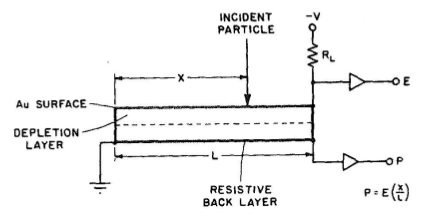
\includegraphics[width=0.8\textwidth]{emsf-09-polpasik.png}
\centering
\caption{Základná konfigurácia pozične citlivého polovodičového detektoru. Signál polohy (P) je získaný oddelením odporového náboja od spodnej vrstvy. E signál je úmerný energii uloženej časticou v aktívnom objeme detektora.}
\label{em9:fig:polpasik}
\end{figure}

\subsection{Mikrostripové polovodičové polohové detektory} 
Alternatívnou pozične citlivou metódou je rozdeliť jednú z elektród na niekoľko nezávislých segmentov alebo pruhov. Keďže vytvorený elektrón-dierový pár v detektore sa pohybuje pozdĺž elektrického poľa k odpovedajúcemu segmentu elektródy, tak silný signál bude odvodený len z tých segmentov, ktoré nazhromažďujú významné množstvo nosičov náboja. Pokiaľ detektorom prejde častica s krátkym dosahom, bude generovaný len jeden takýto signál. Pre častice s dlhším dosahom je nutné interpolovať signály zo susedných segmentov a nájsť strednú hodnotu pozície dráhy danej častice.

Kremíkový mikrostripový detektor je taký, v ktorom bola na jednom povrchu vyrobená séria úzkych rovnobežných páskových elektród s použitím techniky implantácie iónov alebo fotolitografie. Pre dobré priestorové rozlíšenie sa také detektory produkujú s prúžkami tenkými asi $10\: \mu m$. Aby sa zabránilo mnohým nezávislým elektronickým kanálom, ktoré by boli potrebné na meranie signálu z každého pásu nezávisle, boli vyvinuté schémy na nájdenie pásu, ktorý je najbližšie k interakcii, použitím jednorozmerného rozdelenia náboja pozdĺž línie, ktorá spája všetky pásy.

Obojstranné spracovanie kremíkových dosiek môže poskytnúť konfigurácie, ako je znázornená na obrázku (\ref{em9:fig:polpasik}). Elektródové prúžky na opačných stranách dosiek sú navzájom orientované kolmo. Keďže na oboch stranách sa bude indukovať náboj, je možné týmto spôsobom získať x-ovú a y-ovú polohu častice.

\begin{figure}[!h]
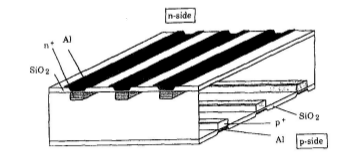
\includegraphics[width=0.7\textwidth]{emsf-09-double.png}
\centering
\caption{Obojstranný kremíkový stripový detektor.}
\label{em9:fig:double}
\end{figure}

\subsection{Pad alebo Pixlový detektor}
Prístup k získaniu dvojrozmernej informácie o polohe interakcie pomocou jednostranného kremíkového detektora je vyrobiť hornú elektródu ako šachovnicový vzor jednotlivých malých elektród, ktoré sú navzájom elektricky izolované. Keď sú rozmery jednotlivých elektród milimetrové a väčšie, tak hovoríme o pad detektoroch. Pri rozmeroch elektród menších ako jeden milimeter hovoríme o pixlovom detektore. Každá elektróda musí mať vlastné elektrické pripojenie a samostatné vyčítacie kanály.

Jednou výhodou tohto prístupu je to, že malá veľkosť každej elektródy vedie k relatívne malej kapacite a malému unikajúcemu prúdu, a tým sa výrazne zníži elektronický šum. V dvoj-dimenzionálnom mikrostripovom detektore máme oveľa väčší elektronický šum. Napríklad, šum meraný pixlovým detektorom môže byť 100 elektrónov na jeden pixel zatiaľčo pre stripový detektor to môže byť 1500 elektrónov.

Zabezpečiť samostatné elektrické pripojenie na každý pixel predstavuje náročnú výzvu. Pri detektoroch s malou plochou, v ktorých sú pixly alebo pad-y dostatočne veľké je možné viesť klasický drôt z každého pixlu na okraj dosky. Avšak, pre dosť malé rozmery pixlov už nie je možné viesť drôt z každého pixlu a preto je potrebné zabezpečiť napájanie iným spôsobom. Najznámejší spôsob ako niečo také dosiahnuť je znázornení na obrázku (\ref{em9:fig:pixel}), kde pixlový detektorový čip je spojený s vyčítacím čipom pomocou tzv. flip chip solder bonding alebo inak indium bump bonds. 

Táto metóda (indium bump bonds) je založená na procese kedy sa spájanie medzi komponentom a substrátom vytvorí nasledovne. Najprv sa zahrievaním roztavia kovové guľôčky a následne sa to spoji stlačením s definovanou lepiacou silou (termokompresia). Spoj sa vytvára pomocou difúzneho zvárania. Na obrázku (\ref{em9:fig:pixel}), v zakrúžkovanej časti je vidieť podstatu tohto spojenia.

Každý vyčitací čip je vyrobený s presne takou istou geometriou rozloženia vyčítacích konektorov akú má pixlový detektor, aby sa každý vyčítací konektor mohol spojiť s jedným pixlom. Pixlové alebo pad detektory majú zvyčajne aktívne oblasti, ktoré sú obmedzené na niekoľko štvorcových centimetrov.

\begin{figure}[!h]
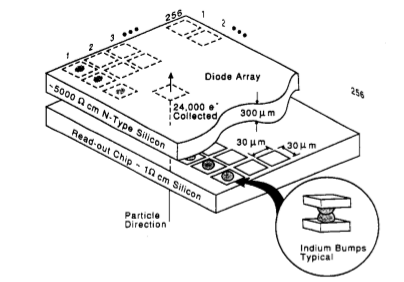
\includegraphics[width=0.7\textwidth]{emsf-09-pixel.png}
\centering
\caption{Hybridný pixlový detektor pozostávajúci z oddeleného detektora a elektronického čipu. Tieto dve komponenty sú navzájom spojené pomocou indium bump bonds technikou.}
\label{em9:fig:pixel}
\end{figure}

\subsection{Driftové polovodičové detektory}
Ukázalo sa, že doba driftu nosičov náboja môže byť v kremíkovom detektore použitá na určenie polohy vzniku týchto nosičov náboja v objeme detektora. V polovodičových driftových detektoroch sa k tomu používa jedinečné usporiadanie elektród, viď obrázok (\ref{em9:fig:drift}). Polovodičové prechody sú vytvorené na oboch stranách waferu, pričom každý je zapojený v závernom smere, až kým detektor nie je úplne vyčerpaný. Elektróny vytvorené ionizujúcim žiarením vo vnútri polovodiča sú viazané v potenciálovej jame a prinútené driftovať v smere rovnobežnom s povrchom waferu. Anóda, čo zbiera elektróny je umiestnená na okraji waferu. Čas potrebný na to, aby sa tieto elektróny posunuli k anóde, je potom lineárnym meraním vzdialenosti medzi anódou a polohou interakcie. Detektory s aktívnou zónou $2.5\,\unit{cm} \times 2.5\,\unit{cm}$ môžu dosahovať priestorové rozlíšenie menšie než $0.5\,\unit{mm}$. Obrázok (\ref{em9:fig:drift}) znázorňuje takzvané lineárne driftové zariadenie, v ktorom sú paralelné pásy použité na tvarovanie poľa a vytvárajú potenciálny gradient potrebný na presun elektrónov na zbernú anódu. V tomto prípade je anóda segmentovaná, aby umožnila určenie súradnice druhej polohy v dimenzii rovnobežnej s pásikmi.

\begin{figure}[!h]
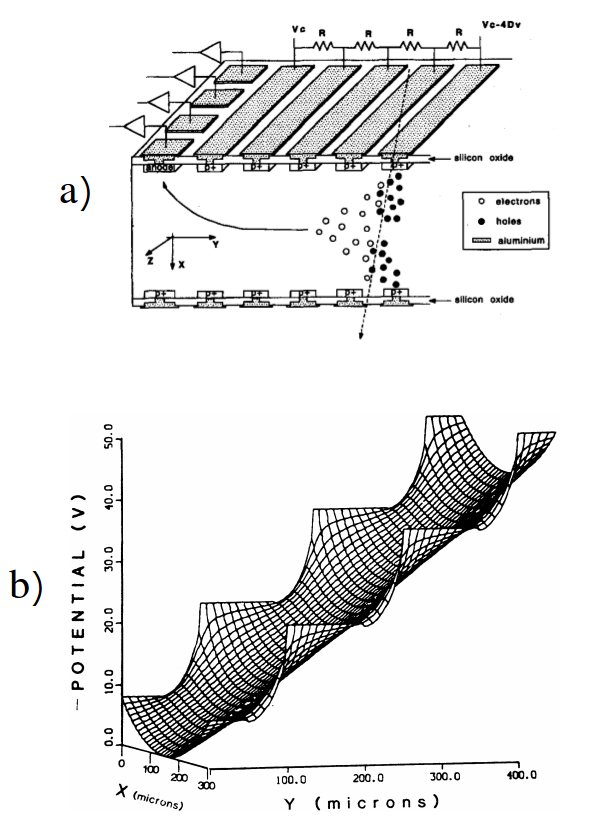
\includegraphics[width=0.7\textwidth]{emsf-09-driftpot.png}
\centering
\caption{(a) Štruktúra lineárneho kremíkového detektora. Elektróny vytvorené ionizujúcim žiarením sú najprv stiahnuté k minimu potenciálu blízko stredu waferu. Následné sú kvôli gradientu potenciálu medzi povrchovými stripmi transportované paralelne s povrchom na anódu na hrane waferu.(b) tvar potenciálu, ktorý vytvoria paralelne pásy na povrchu waferu.}
\label{em9:fig:drift}
\end{figure}

Obrázok (\ref{em9:fig:valecdrift}) znázorňuje valcovú geometriu driftového detektora, v ktorom je zberná anóda umiestnená v strede série krúžkov, ktoré slúžia na účely tvarovania elektrického poľa. V tomto prípade sú všetky ionizujúce elektróny zhromaždené na jednej malej anóde, ktorá je udržiavaná veľmi malá na minimalizáciu jej kapacity. V znázornenom príklade bol integrovaný tranzistor (FET) použitý, aby sa minimalizovala pridaná rozptýlená kapacita, ktorá by zahŕňala spojenie s externým predzosilňovačom. Na obrázku je tiež znázornený výsledný povrchový potenciál pre elektróny, ktorý ilustruje, že elektróny vytvorené kdekoľvek v objeme kremíka sú vedené do malej anódy v strede. Táto konfigurácia poskytuje plochý zadný povrch bez povrchových štruktúr, ktorý môže slúžiť ako tenké vstupné okno pre slabé prenikanie žiarenia.

\begin{figure}[!h]
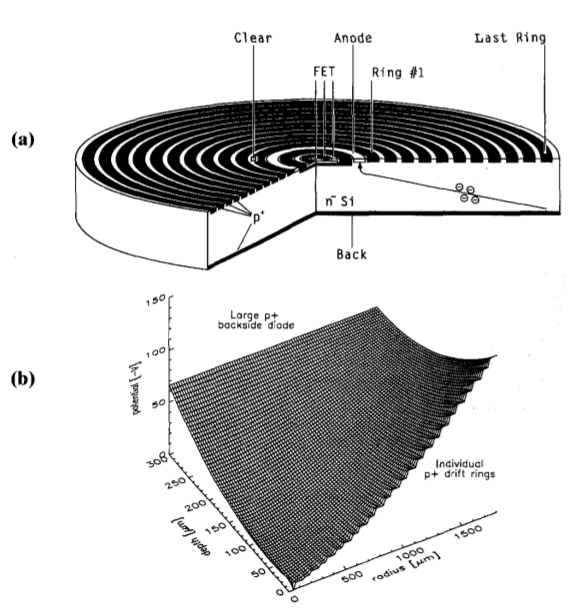
\includegraphics[width=0.8\textwidth]{emsf-09-valecdrift.png}
\centering
\caption{(a) Prierez cylindrického detektora s integrovaným FET pripojeným k zbernej anóde. Neštruktúrovaný zadný povrch detektorov môže poskytnúť tenké vstupné okno pre slabé prenikajúce žiarenia. (b) Povrch potenciálnu pre elektróny pre zariadenie podľa časti (a). Centrálna zberná anóda je zobrazená v blízkom rohu (okolie bodu [0,0]).}
\label{em9:fig:valecdrift}
\end{figure}

Konfigurácia driftového detektora má ďalšiu výhodu, ktorú je možné využiť k zlepšeniu energetického rozlíšenia. Keďže elektróny môžu driftovať dlhé vzdialenosti a byť zozbierané na elektróde veľmi malého rozmeru, môže byť kapacita detektoru omnoho menšia než kapacita ekvivalentnej polovodičovej diódy konvenčného prevedenia. Práve kapacita detektoru je významným faktorom ovplyvňujúcim úroveň šumu spektroskopického systému - nízka kapacita je pritom veľkou výhodou.

\subsection{Nábojovo viazaná štruktúra (CCD)}
Je to označenie pre elektrický jav presunu elektrického náboja po ploche v elektronických (polovodičových) prvkoch. Náboj je prenášaný pomocou sústavy elektród, na ktoré sú privádzané navzájom posunuté synchronizačné signály. Výhody CCD: linearita, veľký dynamický rozsah, nízky šum (2-5 elektrónov), stabilita detektorov, možnosti detekcie širokého spektra vlnových dĺžok. 

CCD boli zavedené začiatkom 70. rokov ako zariadenia ktoré boli schopné zaznamenať viditeľné svetlo. Ich aplikácia sa postupne rozrástla a dnes ich môžme nájsť v širokom spektru optických komponentov a fotoaparátoch. Tieto komerčné aplikácie zostávajú dominantnou ekonomickou silou za vývojom CCD. Avšak menšia podskupina zariadení s podobnými vlastnosťami, často nazývanými vedecké CCD, sa objavila v deväťdesiatych rokoch minulého storočia ako veľmi užitočné senzory na detekciu a zobrazovanie žiarenia. Zistilo sa, že sa dajú použiť pri zobrazovaní dráh vysoko-energetických ionizujúcich častíc.

Schéma jednoduchého CCD snímača je zobrazená na obrázku (\ref{em9:fig:CCD}). Ide zvyčajne o kremíkové štruktúry vyrobené mnohými štandardnými technikami mikroelektroniky, ktoré sa používajú pre integrované obvody. Typické CCD majú štvorčekové plochy s rozmerom $1-2\,\unit{cm}$ a sú zvyčajne vyrábané na kremíkovom wafery, ktorý má hrúbku niekoľko stoviek mikrónov. V štandardnom CCD sa vytvorí oblasť vyčerpania bezprostredne pod predným povrchom zariadenia a potenciálové minimum pre elektróny sa vytvorí niekoľko mikrónov pod povrchovou štruktúrou pozostávajúcou z metal-oxid-silicon (MOS) elektródovej štruktúry. Veľkosť jedného pixelu je približne $25\,$mikrónov. 

\begin{figure}[!h]
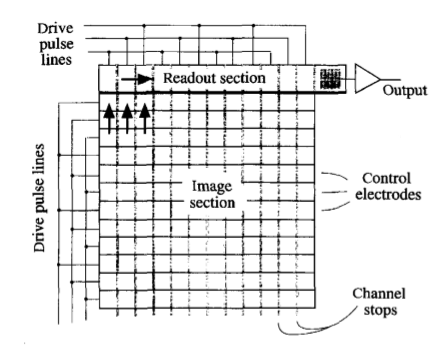
\includegraphics[width=0.8\textwidth]{emsf-09-CCD.png}
\centering
\caption{(Rozloženie povrchu CCD senzora.}
\label{em9:fig:CCD}
\end{figure}

Alternatívnym prístupom je nahradenie metal-oxid elektródy s p-n diódovou štruktúrou na povrchu, viď obrázok (\ref{em9:fig:CCDpn}), s väčšími typickými rozmermi pixlov $150\,$ mikrónov. Plocha CCD senzorov je rozdelená na veľké množstvo malých pixlov skrz kontrolne elektródy, viď obrázok (\ref{em9:fig:CCD}). Akonáhle je na kontrolnej elektróde aplikované napätie, na každom pixly sa vytvoria potenciálové jamy, v ktorých sa nahromadia všetky voľné elektróny vytvorené ionizujúcim žiarením. CCD je teda neoddeliteľne integračným zariadením, ktoré zhromažďuje náboje v pixloch, ktoré sa jednoducho akumulujú počas doby expozície. Pre lepšiu predstavu si poďme princíp fungovania CCD poriadne načrtnúť.

\begin{figure}[!h]
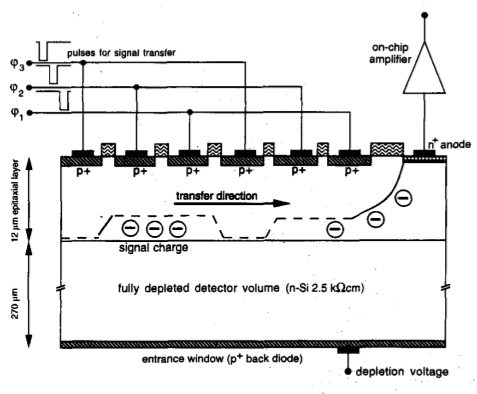
\includegraphics[width=0.8\textwidth]{emsf-09-CCDpn.png}
\centering
\caption{(Prierez cez transportný kanál pn-CCD senzora.}
\label{em9:fig:CCDpn}
\end{figure}

CCD snímač využíva, podobne ako všetky ostatné svetlocitlivé súčiastky, fyzikálny jav známy ako fotoefekt. Tento jav spočíva v tom, že častice svetla pri náraze do atómu dokážu uvoľniť nejaký elektrón z atómu. V polovodiči sa takto uvoľnený elektrón odvedie pomocou elektród. V CCD je však elektróda od polovodiča izolovaná tenučkou vrstvou oxidu kremičitého (SiO$_2$), ktorý sa chová ako dokonalý elektrický izolant, takže fotoefektom uvoľnené elektróny nemôžu byť odvedené preč. Činnosť CCD sa skladá z troch fáz:

1.) V tejto fáze sú z CCD bez prístupu svetla odobraté všetky voľné elektróny, čím sa z neho vymažú všetky zvyšky predchádzajúceho obrazu.

2.) Expozícia obrazu: Na elektródy označené na obrázku číslom 1 (viď obrázok \ref{em9:fig:CCD1}), sa privedie kladné napätie a na CCD sa nechá pôsobiť svetlo (napríklad v digitálnom fotoaparáte sa otvorí uzávierka). Dopadajúce fotóny excitujú v polovodiči elektróny, ktoré sú potom priťahované ku kladne nabitým elektródam. Po elektrónoch ostanú v polovodiči tzv. diery, ktoré voči svojmu okoliu vykazujú kladný náboj a sú priťahované elektródou na spodnej strane CCD. Hranice pixlov sú na obrázku znázornené zvislými bodkovanými čiarami. Pretože na pixel vľavo dopadlo viac fotónov, zhromaždilo sa u jeho elektródy viac elektrónov, než na pixly vpravo.

\begin{figure}[!h]
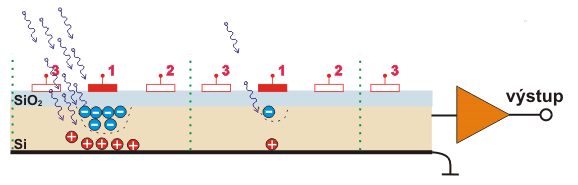
\includegraphics[width=0.8\textwidth]{emsf-09-CCD1.png}
\centering
\caption{Princíp fungovania CCD 2. fáza.}
\label{em9:fig:CCD1}
\end{figure}

3.) Odčítanie obrazu: Po zavretí uzávierky sa začnú na skupiny elektród rovnakého čísla privádzať synchronizované impulzy. To znamená, že na elektródach 2 sa začne pozvoľna zvyšovať napätie, zatiaľ čo na elektródach 1 sa súbežne zníži. Vďaka tomu sú skupiny elektrónov priťahované pod elektródy 2. Impulz sa posunie na ďalšiu elektródu a elektróny ho poslušne nasledujú. Následne sa celý dej opakuje, až kým sa skupiny nazhromaždených elektrónov neodčítajú všetky, viď obrázok (\ref{em9:fig:CCD2}). Odpočet sa deje na konci čipu, kde je výstupný zosilňovač. Ten zosilní pomerne malý elektrický náboj, zodpovedajúci počtu nachytaných elektrónov v jednotlivých pixloch, na úroveň vhodnú pre ďalšie spracovanie obrazu.

\begin{figure}[!h]
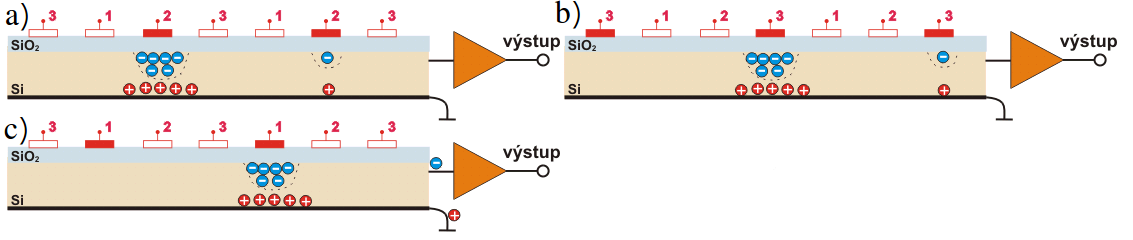
\includegraphics[width=1.0\textwidth]{emsf-09-CCD2.png}
\centering
\caption{Princíp fungovania CCD 3. fáza.}
\label{em9:fig:CCD2}
\end{figure}

Toto jednoduché vyčítanie je dôvodom popularity týchto senzorov. Na obrázku (\ref{em9:fig:CCD}) môžme vidieť ako také vyčítanie prebieha. V tomto obrázku sú náboje akumulované v hornej časti CCD (tie čierne šípky). Podľa vyššie spomenutého princípu sa elektróny presunú do Readout sekcie, v ktorej sa taktiež tým istým princípom budu pohybovať smerom k výstupovému zosilňovaču. Tento proces pokračuje, kým sa celý riadok nevyčíta postupne. Potom driven line pulses v imaging section opäť sa nastavia tak, aby posunuli každý riadok o krok nahor a proces výčítania sa opakuje. Efektivita prenosu náboja z jednej potenciálovej jamy do druhej je v CCD senzoroch veľmi dobrá a v najlepších zariadeniach tohto druhu sa náboje vôbec nestrácajú, ani pokiaľ tieto senzory podstúpia tisícky prenosov.

Vyčítací zosilňovač má extrémne nízku kapacitu, preto je možné pri malej úrovni šumu rozlíšiť i malé balíčky nábojov. Na druhej strane môžu ako zdroj šumu slúžiť elektróny termálne generované vo vnútri kremíka - toto je obzvlášť v senzoroch, ktoré používajú široké ochudobnené oblasti, veľký počet pixlov, a dlhé expozičné doby. K redukcii tohto tepelného šumu sa doporučuje ochladiť senzor približne o $50-100^{\circ}$ oproti izbovej teplote. Zatiaľ čo ide o zjavnú prevádzkovú komplikáciu, je menej náročná než kvapalné dusíkové chladenie vyžadované hrubými Si(Li) detektormi. Keďže plocha senzora môže obsahovať $10^6$ a aj viac pixlov, vyčítacie doby sa môžu pohybovať na úrovni okolo jednej sekundy. Sú však už metódy, ktoré tieto časy skrátia.

\subsection{Priestorové rozlíšenie detektorov} 
Detektor poskytuje informáciu o tom, či nastal hit alebo či nenastal hit. Hit môže nastať hocikde vo vnútri pixlovho poľa. Pravdepodobnostné rozdelenie toho, že nastane hit v pixly, je 
$$ f(x) = \frac{1}{p} $$

\begin{figure}[!h]
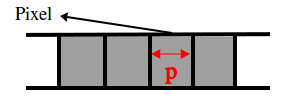
\includegraphics[width=0.5\textwidth]{emsf-09-rozlisenie.png}
\centering
\caption{Pravdepodobnostné rozlíšenie v jednom pixly.}
\label{em9:fig:rozlisenie}
\end{figure}

Potom stredná hodnota polohy hitu bude 
$$ \mu = \int_0^p \frac{1}{p}x dx  = \frac{p}{2}.$$
Pre rozptyl píšeme 
$$ \sigma^2 = \int_0^p (x-\mu)^2 \frac{1}{p}dx = \frac{p^2}{12} \rightarrow \sigma = \frac{p}{\sqrt{12}}.$$

\section{TPC - časovo projekčná komora}
Časová projekčná komora (TPC) je typ detektora častíc, ktorý používa kombináciu elektrických polí a magnetických polí spolu s citlivým objemom plynu alebo kvapaliny na vykonanie trojrozmernej rekonštrukcie trajektórie častíc alebo interakcii. 3D zobrazenie umožňuje kombinácia driftovej komory, z ktorej získame časovú informáciu a dvoj-dimenzionálnych mnoho-vláknových proporcionálnych komôr, z ktorých získame pozíciu v 2D. Keď daný detektor umiestnime do magnetického poľa tak sme schopný merať hybnosť častíc.

Žiarenie prechádzajúce cez objem detektora vytvorí ión-elektrónové páry. Tieto nabité častice ihneď po svojom vzniku začnú driftovať prostredníctvom elektromagnetického poľa k čítacím detektorom umiestneným na konci TPC. Elektrické pole je zvolené tak, aby nedochádzalo k rekombinácii ale ani k multiplikácii náboja. Presnosť určenia polohy častice býva na úrovni $0.5\,\unit{mm}$ a rýchlosť TPC býva určená rýchlosťou driftu a ten je na úrovni $100\,\unit{\mu s}$. Pomocou tohto detektora je možné určiť aj druh častice pomocou energetických strát d$E$/d$x$.

V ďalších úvahách budeme opisovať TPC, ktoré sa nachádza na experimente STAR. TPC je časť STAR detektora, ktorá zaznamenáva dráhy častíc, meria ich hybnosti a identifikuje častice pomocou ionizačných energetických strát (d$E$/d$x$). Jeho pseudo-rapidita pokrýva rozsah $-1.8 < \eta <1.8$ s plne azimutálnym pokrytím. Častice sú merané v rozsahu $100\,\unit{MeV}/c - 30\,\unit{GeV}/c$. TPC detektor je umiestnený vo veľkom solenoidovom magnete, ktorý pracuje pri $0,5\,\unit{T}$. Obklopuje oblasť interakcie a jeho driftový objem je obmedzený dvomi súosovými valcami s polomermi $50\,\unit{cm}$ a $200\,\unit{cm}$ s dĺžkou $4,2\,\unit{m}$, viď obrázok (\ref{em9:fig:STAR}). 

\begin{figure}[!h]
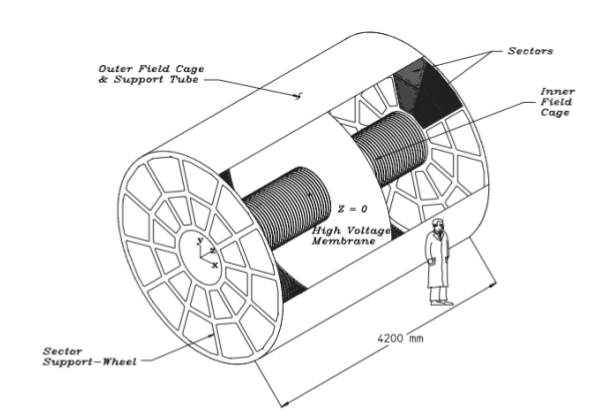
\includegraphics[width=0.7\textwidth]{emsf-09-STAR.png}
\centering
\caption{Schéme detektora TPC z experimentu STAR.}
\label{em9:fig:STAR}
\end{figure}

Dráhy primárnych ionizujúcich častíc, ktoré prejdu cez objem plynu, sa rekonštruujú s vysokou presnosťou z uvoľnených sekundárnych elektrónov, ktoré driftujú do odčítavacích časti, ktoré sú umiestnene na koncoch komory (v obrázku \ref{em9:fig:STAR} sú to tie veci nazvané Sectors). Jednotné elektrické pole, ktoré sa vyžaduje na presun elektrónov je definované tenkou vodivou membránou v strede TPC, sústrednými field-cage valcami a readout koncovými uzávermi.

TPC detektor je naplnený plynom P10 ($10\%$ metán, $90\%$ argón) regulovaným pri atmosférickom tlaku $2\,\unit{mbar}$ a plyn cirkuluje rýchlosťou $36 000\,\unit{l/h}$ (plný objem TPC je $50 000\,\unit{l}$). Hlavnou vlastnosťou tohto plynu je rýchla driftová rýchlosť, ktorá dosahuje vrchol pri nízkom elektrickom poli. Centrálna membrána je udržiavaná na hodnote $28\,\unit{kV}$, ktorá spolu s ekvipotenciálnymi krúžkami pozdĺž vnútornej a vonkajšej klietky vytvára rovnomerné unášacie pole $135\,\unit{V/cm}$ od centrálnej membrány k uzemneným koncovým uzáverom, kde sú umiestnené čítacie komory.

Systém vyčítania je založený na multi-drôtových proporcionálnych komorách (MWPC) a pozostáva z 12 sektorov. Každý sektor je rozdelený na vnútorný a vonkajší subsektor, viď obrázok \ref{em9:fig:pad}. Vonkajší subsektor (obsahuje 32 radov tvorených z pad-ov) má úplné pad pokrytie pre lepšie d$E$/d$x$ rozlíšenie a obsahuje 3942 pad-ov. Vnútorný subsektor (13 radov padov) je navrhnutý pre lepší tracking a obsahuje 1750 pad-ov.

\begin{figure}[!h]
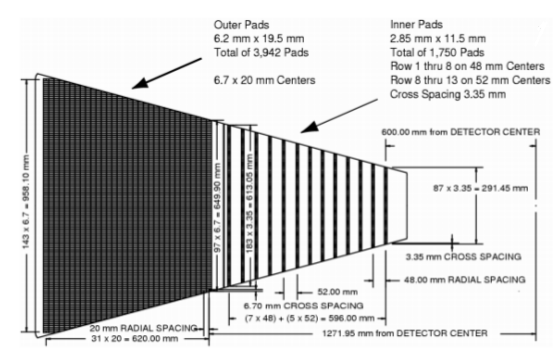
\includegraphics[width=0.7\textwidth]{emsf-09-pad.png}
\centering
\caption{Anódová pad rovina s jedným plným sektorom. Vnútorný podsektor je napravo a má malé pads usporiadané v široko rozmiestnených riadkoch. Vonkajší podsektor je naľavo a pad-y sú hustejšie na sebe.}
\label{em9:fig:pad}
\end{figure}

Ionizujúce elektróny sa posúvajú smerom ku koncovým uzáverom konštantnou rýchlosťou $5.45\,\unit{cm/\mu s}$ a preto je maximálny čas driftu v TPC je $\sim \unit{40\,\mu s}$, čo je aj limita vyčítania. Elektrónové lavíny, ktoré vznikajú v tesných blízkostiach anód, okolo ktorých sa nachádza veľké elektrické pole, poskytujú zosilnenie od 1000 do 3000. Vzniknuté náboje z lavíny sa potom zbierajú pomocou niekoľkých readout pad-ov.

Strata energie v plyne TPC je cenným nástrojom na identifikáciu častíc. Identifikácia funguje dobre pre častice s nízkou hybnosťou, ale so zvyšujúcou sa energiu častíc, energetické straty prestavajú byť primárne závisle na hmotnosti častice, viď obrázok (\ref{em9:fig:dEdx}). Preto je potom ťažké rozoznať častice s rýchlosťami $v> 0,7\,c$. STAR je schopný oddeliť pióny, kaóny a protóny s veľmi dobrou presnosťou až do $1,2\,\unit{GeV}/c$. Energetické straty nabitých častíc sa vypočítajú pomocou Bethe-Bloch formuly.

\begin{figure}[!h]
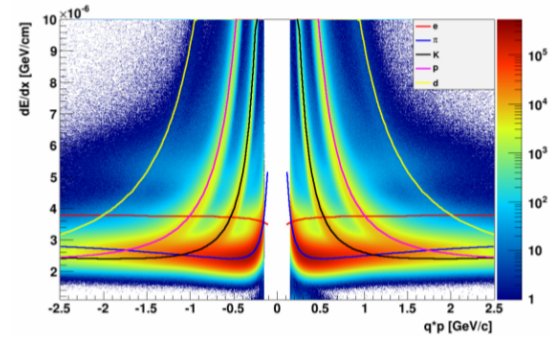
\includegraphics[width=0.7\textwidth]{emsf-09-dEdx.png}
\centering
\caption{Distribúcia energetických strát v TPC ako funkcia hybnosti častíc.}
\label{em9:fig:dEdx}
\end{figure}

\section{TOF - time of flight detektor}
TOF je detektor častíc, ktorý môže rozlišovať medzi ľahšími a ťažšími elementárnymi časticami s rovnakou hybnosťou s použitím času ich letu.
Ako sme spomínali vyššie, identifikácia častíc sa na STAR experimente vykonáva prostredníctvom TPC detektora. Avšak TPC má problém identifikovať nabité hadróny, ak ich hybnosť presahuje $\sim 0,6\,\unit{GeV}/c$, pretože sa začnú vzájomne miešať energetické pásy, ako môžme vidieť na obrázku (\ref{em9:fig:dEdx}). Preto bol TOF detektor s celkovým časovým rozlíšením $100\,\unit{ps}$ vyvinutý, aby zlepšil identifikáciu častíc na experimente STAR, pre častice s hybnosťami v rozmedzí $0,6-3\,\unit{GeV}/c$. TOF detektor sa nachádza hneď za TPC, prakticky by sme mohli povedať, že TOF tvorí TPC detektoru akýsi obal.

Detektor TOF má valcový tvar, pokrývajúci polárne uhly medzi 45$^\circ$ a 135$^\circ$, tj. pokrýva pseudo-rapiditu $-1 < \eta < 1$, a tiež celý azimut. Systém je založený na Multi-gap Resistive Plate Chamber (MRPC) technológii. Má modulárnu štruktúru so 120 sektormi. Avšak, týchto 120 sektorov je rozdelených na 60 a 60, pretože dĺžka týchto sektorov siaha len do polovice TPC. Takže okolo jednej polovice TPC máme 60 sektorov. Ďalej, každý tento modul obsahuje 32 MRPC stripov a logicky pokrýva 6 stupňov v azimute a jednotku v pseudo-rapidite. Na obrázku \ref{em9:fig:TOF} máme znázornený TOF detektor pre experiment ALICE, lebo bolo nemožné nájsť TOF detektor pre experiment STAR. Podstata sa však nelíši.

\begin{figure}[!h]
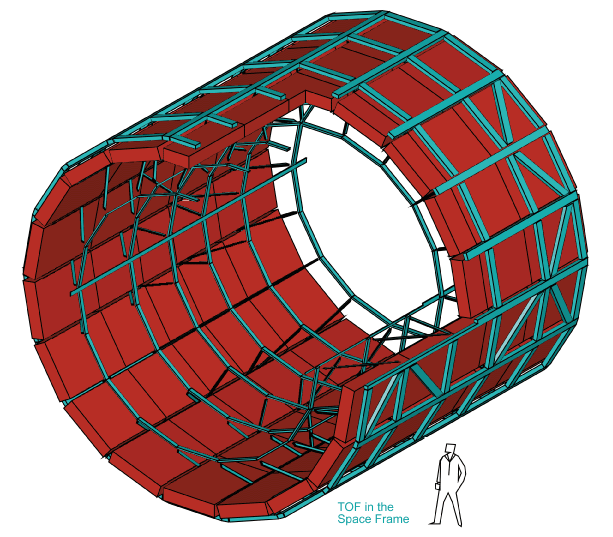
\includegraphics[width=0.4\textwidth]{emsf-09-TOF.png}
\centering
\caption{Geometria TOF detektoru pre experiment ALICE. Vidíme, že TOF sa skladá z 18 sektorov, každý sektor je rozdelený do 5 modulov pozdĺž smeru zväzku. Moduly spolu obsahujú 1638 detektorových elementov (MRPC stripov).}
\label{em9:fig:TOF}
\end{figure}

Princíp fungovania MRPC stripu je nasledovný. MRPC je tvorený súborom rezistentných sklenených dosiek, ktoré sú zoradené paralelne vedľa seba, viď obrázok \ref{em9:fig:MRPC}. Z vonkajšej strany MRPC stripu sú dve zberné elektródy, na ktorých je privedené vysoké elektrické napätie. Pri prechode nabitej častice cez MRPC vzniknú ionizáciou voľné elektróny, ktoré pod vplyvom vysokého napätia začnú zrýchľovať smerom k elektródam a vzniknú tak elektrónové lavíny. Rezistentné sklenené platne zastavujú rozvoj lavíny v každej medzere, sú však transparentné pre rýchly signál indukovaný na snímacích elektródach pohybom elektrónov. Takže celkový signál je súčtom signálov zo všetkých medzier (dôvodom mnohých medzier je dosiahnutie vysokej účinnosti).

\begin{figure}[!h]
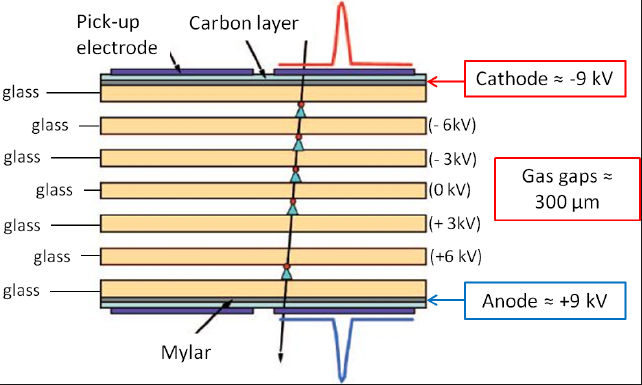
\includegraphics[width=0.6\textwidth]{emsf-09-MRPC.png}
\centering
\caption{Princíp fungovania MRPC stripu.}
\label{em9:fig:MRPC}
\end{figure}

Na základe informácii z TOF detektora je relatívna rýchlosť ($\beta$) častice daná vzťahom
$$ \frac{1}{\beta} = \frac{c\tau}{L}, $$
kde $\tau$ je doba letu častice, ktorú urči práve TOF detektor, $L$ je dĺžka dráhy častice a $c$ je rýchlosť svetla.
Z relativistickej hybnosti častice získavame (v natural units)
$$ p = m \beta \gamma  \rightarrow p^2 = \beta^2 (m^2+p^2),$$
kde $m$ je hmotnosť častice, ktorú nevieme. Výsledný vzťah podľa, ktorého určime hmotnosť častice je
$$ \frac{1}{\beta} = \sqrt{\bigg( \frac{m^2}{p^2}+1 \bigg)},$$
kde poznáme všetko okrem hmotnosti. Hybnosť $p$ sa určí pomocou TPC.

\end{document}